% This document is going to serve as a list of definitions for the work that I am doing in
% topological signal processing. This is going to be a living document that I will update it as I
% learn more useful things.

\documentclass[12pt]{article}
\author{Mauricio Montes}

\usepackage{amsmath, graphicx, amssymb}

\title{Topological Signal Processing Definitions}

\begin{document}

\maketitle

\section{Introduction}

This document is for me to keep track of the definitions and ideas I have about topological signal
processing. This will probably get long, so maybe we can chunk it later. I'm not sure if I want to
start all the way with the definition of a topological space. But I think I can start with the ideas
of homology and cohomology. 

\section{Definitions}

\subsection{Simplicial Homology}

The central objects of simplicial homology are simplicial complexes.

\begin{itemize}

\item A k\textbf{-simplex} is the convex hull of a set of $k+1$ points in some Euclidean space. We can think of a 0-simplex as a
  vertex. A 1-simplex is an edge, a 2-simplex is a triangle, and so on. 

\item Note that a k-simplex has $k+1$ faces, which are the simplices of dimension $k-1$ that are
  contained in it.

\item A \textbf{simplicial complex} is a collection of simplices such that the intersection of any two simplices is either empty or
another simplex.

\item The \textbf{dimension} of a simplicial complex is the maximum dimension of any of the simplices in the complex. 

\end{itemize}

In order to do algebra with simplicial complexes, we need to associate it to algebraic objects that
we can manipulate. This is where the chain complex comes in.

\begin{itemize}

  \item Say $X$ is a $k$-dimensional simplicial complex. The \textbf{chain group} $C_k(X,
    \mathbb{R})$ is the vector space (over $\mathbb{R}$) with basis given by the number of
    $k$-simplices in $X$. 

\end{itemize}

\begin{figure}[ht]
  \begin{center}
      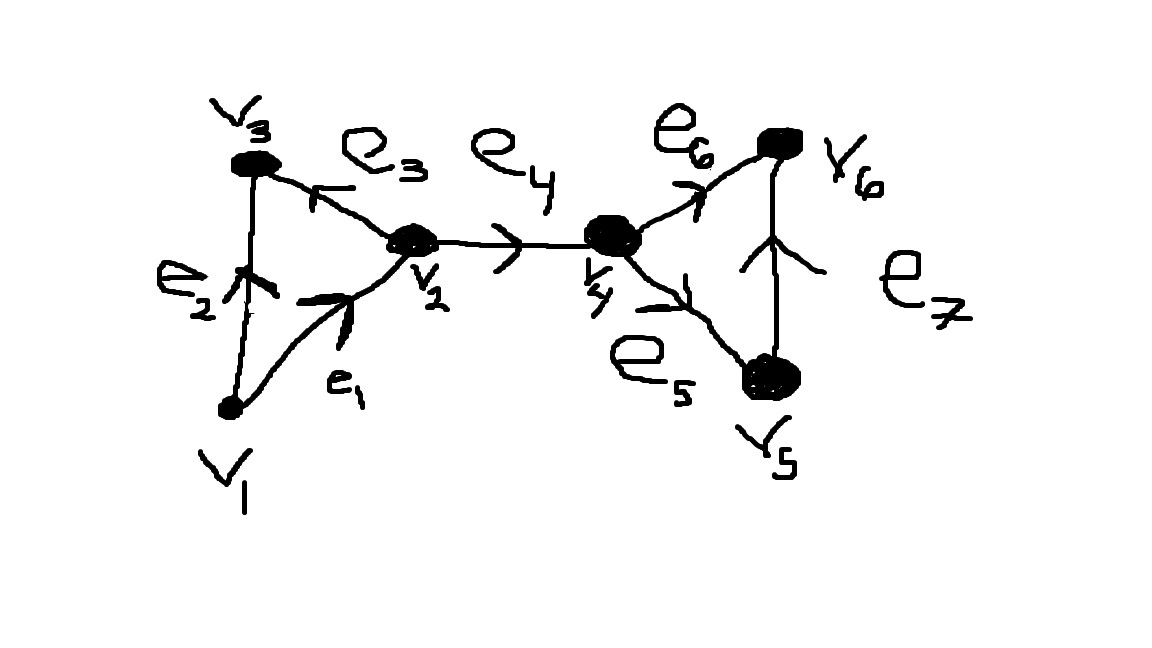
\includegraphics[width=0.5\textwidth]{Simp_Cx.jpg}
  \end{center}
\caption{A simplicial complex, with 6 vertices and 7 edges.}
\end{figure}

Inspecting the image, we see that we have two 

\end{document}
